\section{Experiments}
\label{sec:exp}

We now test the method step by step. The questions follow the four problems
of \cref{sec:intro}: does the classifier work on new people, does the filter
stop the shake, does voting stop false clicks, and does the knuckle stop the
jump?

\subsection{Dataset and setup}
\paragraph{Our dataset.} No public dataset has our 7 control gestures together
with hand points, so we recorded our own with our tool
\texttt{collect\_data.py}. Each of the three group members recorded every
gesture while moving the hand around the image, closer and farther, and a
little tilted. In total we have \textbf{15,378 labelled frames} (4,774 to 5,367
per person and 1,880 to 2,530 per gesture), each with its 21 hand points and
handedness, plus \textbf{7,692 hand-crop images} for the CNN baseline.

\paragraph{Two kinds of test.} In the \emph{random split}, 20\% of all frames
are kept for testing. The same people appear in training and testing, so this
test is easy. In \emph{leave-one-user-out}, we train on two people and test
on the third, for each person in turn. This is the honest test, because it is
exactly what happens when a new person uses the system.

\paragraph{Live sessions.} For the cursor experiments we ran the app and saved
every frame's raw hand points and predictions to a log. We recorded three
one-minute sessions: holding the hand still, moving the cursor around, and
pinching exactly 30 times. Because the raw data is saved, we can replay the
\emph{same} hand motion through every filter or voting setting and compare them
fairly.

\paragraph{Implementation.} Python with OpenCV~\cite{bradski2000opencv},
MediaPipe, PyTorch~\cite{paszke2019pytorch}, scikit-learn and
PyAutoGUI~\cite{pyautogui}. The MLP is trained with
AdamW~\cite{loshchilov2019adamw} (learning rate $10^{-3}$, cosine schedule,
label smoothing 0.05~\cite{szegedy2016rethinking}) for 60 epochs with batch
size 64. We keep the epoch with the best validation accuracy. Everything runs on
\Hardware; timings are for one frame on one CPU thread.

\subsection{Can it recognise the gestures?}
\label{sec:exp-cls}

\begin{table}[t]
\centering\small
\caption{Gesture classification on the random 20\% test split (accuracy and macro-F1 in \%, latency per sample on one CPU thread).}
\label{tab:ablation}
\resizebox{\ifdim\width>\linewidth\linewidth\else\width\fi}{!}{%
\begin{tabular}{@{}lcccc@{}}
\toprule
Method & Acc. & F1 & ms & Params \\
\midrule
Rule-based (fingers up) & 89.89 & 90.04 & 0.033 & -- \\
SVM (RBF), our features & 99.74 & 99.74 & 0.150 & -- \\
Random Forest, our features & \textbf{99.84} & \textbf{99.84} & 10.871 & -- \\
kNN ($k$=5), our features & 99.77 & 99.78 & 1.630 & -- \\
\midrule
MLP, raw coordinates & 99.67 & 99.67 & 0.222 & 17.3k \\
MLP, + mirror/translate/scale & 99.80 & 99.80 & 0.293 & 17.3k \\
MLP, + rotation & 99.80 & 99.80 & 0.317 & 17.3k \\
MLP, full features, no augm. & 99.77 & 99.78 & 0.776 & 20.5k \\
\textbf{MLP, full features + augm. (ours)} & 99.74 & 99.74 & 0.720 & 20.5k \\
\bottomrule
\end{tabular}}
\end{table}


\Cref{tab:ablation} shows the random split. The usual rule-based method gets
89.9\%. Every learned method gets between 99.7\% and 99.8\%, and our MLP takes
only 0.72\,ms per frame. On this easy test the learned methods are all about
equally good, and the confusion matrix (\cref{fig:cm}) shows almost no
mistakes. The cleaning steps and augmentation change little here, because
the test frames come from the same people as the training frames.

\begin{figure}[t]
  \centering
  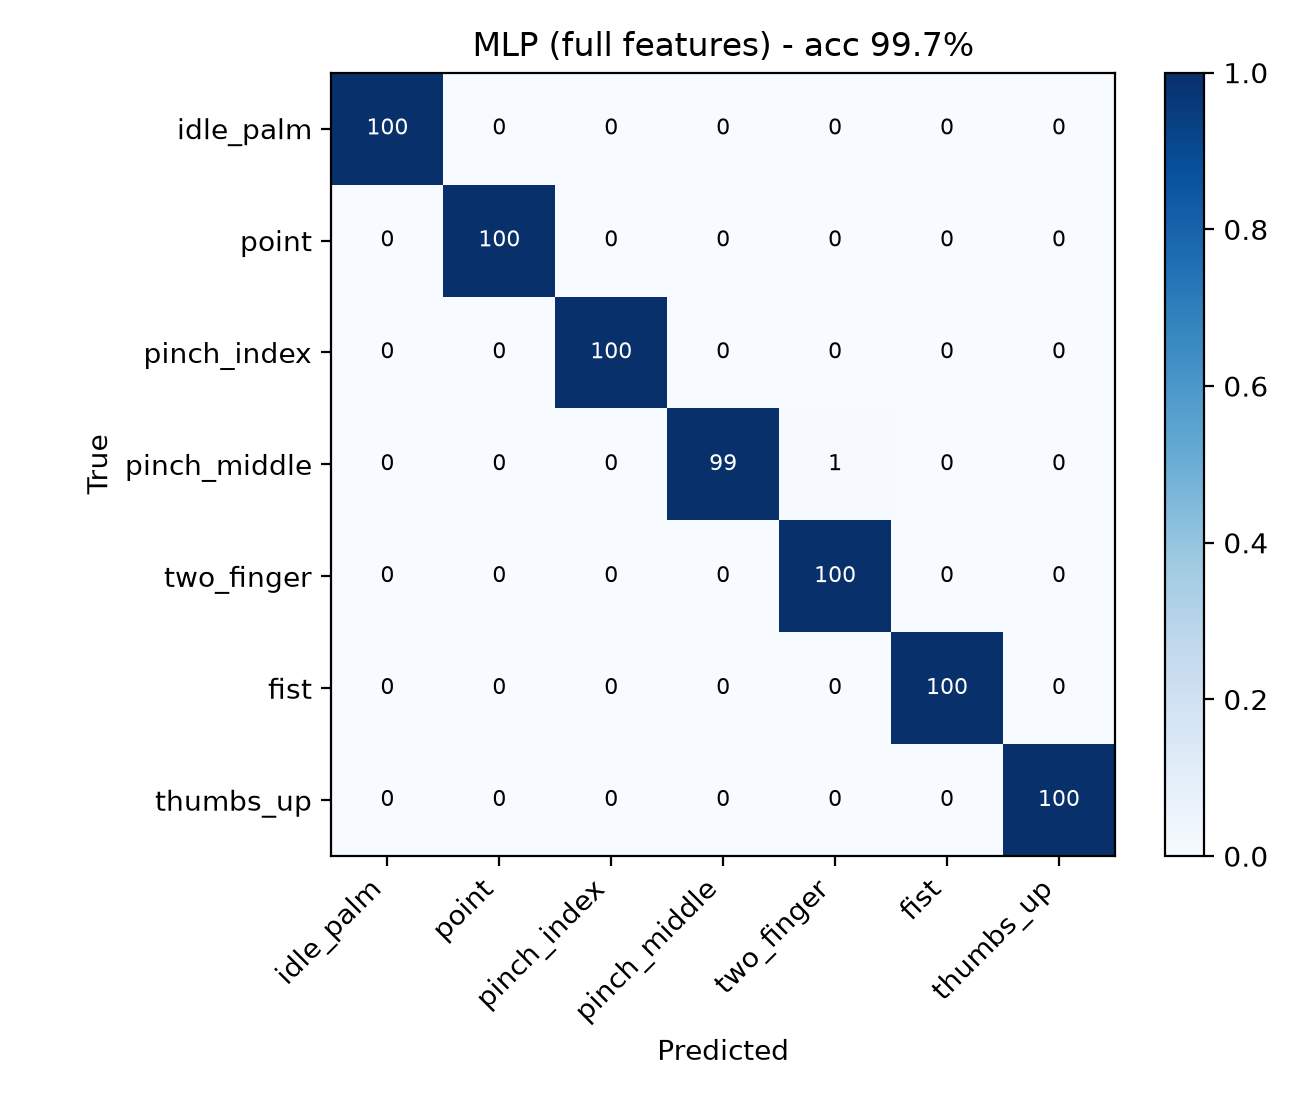
\includegraphics[width=0.9\linewidth]{figures/confusion_matrix.png}
  \caption{Confusion matrix (\%) of our MLP on the random test split.}
  \label{fig:cm}
\end{figure}

\paragraph{The real test: a new person.} \Cref{tab:loso} tells a different
story. When the person is new, the rules drop to 89.8\% and the SVM drops to
90.2\%, with only 76.5\% for Bhuvana's hand. An MLP on the raw points
without augmentation reaches 93.9\%. Our cleaned features with augmentation
reach \textbf{96.6\%} on average, and are the best for two of the three
people. So the cleaning and augmentation pay off exactly where they are needed:
on hands the model has not seen.

\begin{table}[t]
\centering\small
\caption{Leave-one-user-out accuracy (\%): trained on the other users, tested on the user in the row.}
\label{tab:loso}
\resizebox{\ifdim\width>\linewidth\linewidth\else\width\fi}{!}{%
\begin{tabular}{@{}lcccc@{}}
\toprule
Test user & Rules & SVM & MLP raw & MLP ours \\
\midrule
bhuvana & 85.15 & 76.50 & 91.24 & 94.39 \\
guna & 93.50 & 99.05 & 95.73 & 98.30 \\
raj & 90.85 & 95.04 & 94.65 & 97.23 \\
\midrule
\textbf{Mean} & \textbf{89.83} & \textbf{90.19} & \textbf{93.88} & \textbf{96.64} \\
\bottomrule
\end{tabular}}
\end{table}


\paragraph{Hand points or image pixels?} \Cref{tab:cnn} compares our MLP with
a CNN trained on the hand-crop images of the same frames. The CNN is
slightly more accurate on the random split (99.94\% vs.\ 99.74\%). However, it
is about 5.5 times slower (4.0\,ms vs.\ 0.72\,ms per frame), 12 times bigger
(242\,k vs.\ 20\,k weights), and took 455\,s to train. For a system that
must leave time for tracking and control in every frame, the small keypoint
MLP is the better choice.

\begin{table}[t]
\centering\small
\caption{Classifier on image pixels vs.\ on keypoints (same frames, random split).}
\label{tab:cnn}
\resizebox{\ifdim\width>\linewidth\linewidth\else\width\fi}{!}{%
\begin{tabular}{@{}lcccc@{}}
\toprule
Input / model & Acc. & F1 & ms & Params \\
\midrule
CNN, $64\times64$ hand image & \textbf{99.94} & \textbf{99.94} & 4.01 & 242k \\
MLP, keypoint features (ours) & 99.74 & 99.74 & 0.72 & 20.5k \\
\bottomrule
\end{tabular}}
\end{table}


\paragraph{Does personalization help?} \Cref{fig:personal} shows the accuracy
on a new user when only the last layer is re-trained with $K$ samples per
gesture. Averaged over the three of us it rises from 97.4\% ($K=0$) to
98.0\% ($K=20$). The gain is largest for the hardest user, Bhuvana: from
94.8\% to 96.7\% with 20 samples and 97.2\% with 50. For the other two, who
already started near 98--99\%, it changes little.

\begin{figure}[t]
  \centering
  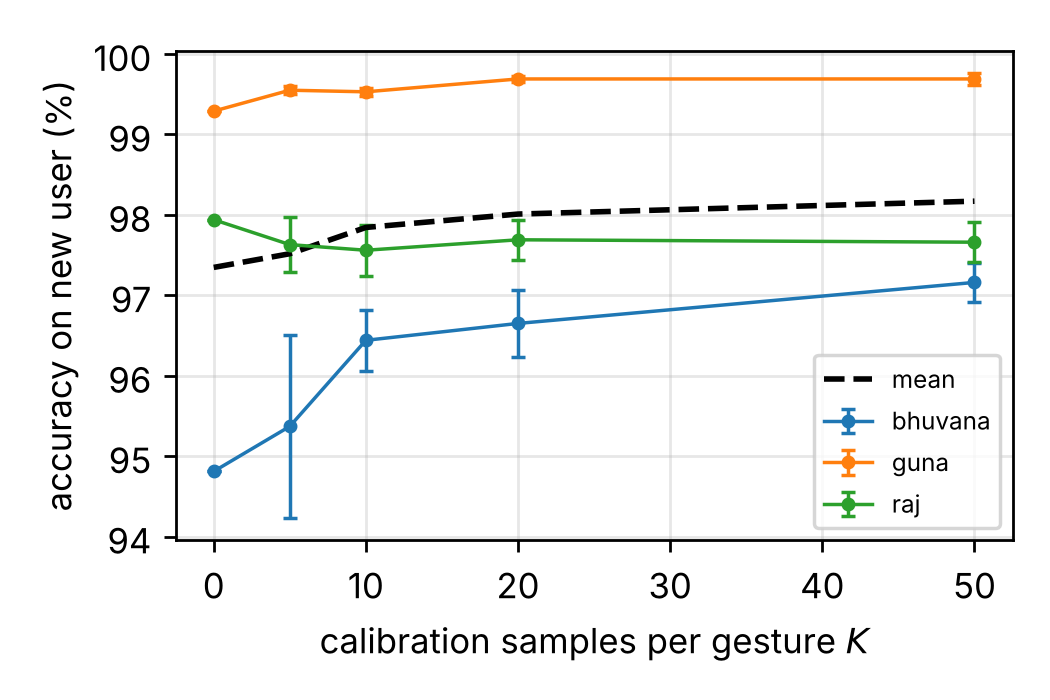
\includegraphics[width=0.85\linewidth]{figures/personalization.png}
  \caption{Accuracy on a new user against the number of calibration samples
  per gesture $K$ ($K=0$ means no calibration).}
  \label{fig:personal}
\end{figure}

\subsection{Is the cursor steady?}
\label{sec:exp-filter}
We replayed the recorded hand motion through four filters
(\cref{tab:filter,fig:trace}). \emph{Shake} is how far the cursor moves per
frame while the hand is held still. \emph{Lag} is how late the filtered cursor
is compared with the intended path.

\begin{table}[t]
\centering\small
\caption{Cursor smoothing on the same recorded hand motion (lower is better for all columns).}
\label{tab:filter}
\resizebox{\ifdim\width>\linewidth\linewidth\else\width\fi}{!}{%
\begin{tabular}{@{}lccc@{}}
\toprule
Filter & Jitter (px/frame) & Error moving (px) & Lag (ms) \\
\midrule
No filter (raw) & 4.21 & \textbf{15.19} & \textbf{0.00} \\
Moving average (5) & 3.57 & 61.52 & 64.03 \\
Kalman (const. velocity) & 3.66 & 37.64 & 32.02 \\
\textbf{One-Euro (ours)} & \textbf{2.59} & 18.82 & 10.65 \\
\bottomrule
\end{tabular}}
\end{table}


Without a filter the cursor shakes by 4.21\,px every frame. The moving
average reduces this only to 3.57\,px and adds 64\,ms of lag, so the cursor
feels like it is pulled on a rubber band. The Kalman filter is in between. The
One-Euro filter gives the \textbf{least shake (2.59\,px, 38\% less than no
filter)} with only \textbf{11\,ms} of lag. Its error while moving (18.8\,px) is
also close to the raw cursor's, while the moving average is far behind
(61.5\,px).

\begin{figure}[t]
  \centering
  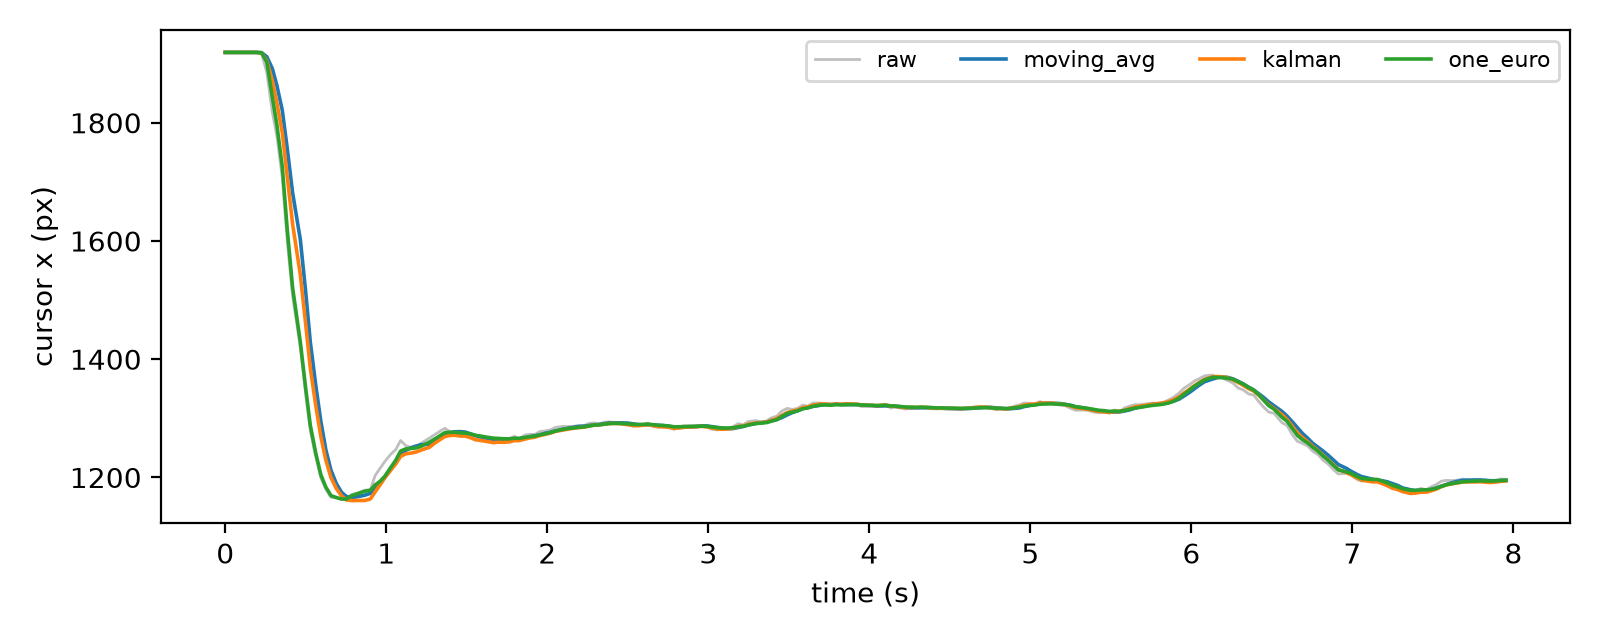
\includegraphics[width=\linewidth]{figures/filter_trace.png}
  \caption{Cursor $x$-position over time in a recorded session: raw and
  filtered.}
  \label{fig:trace}
\end{figure}

\subsection{Does voting stop false clicks?}
In the third session the user pinched exactly 30 times. We replayed the
network's frame-by-frame predictions with and without voting
(\cref{tab:voting}).

\begin{table}[t]
\centering\small
\caption{Effect of temporal voting on the same recorded predictions (the user clicked 30 times).}
\label{tab:voting}
\resizebox{\ifdim\width>\linewidth\linewidth\else\width\fi}{!}{%
\begin{tabular}{@{}lccc@{}}
\toprule
Setting & Changes/min & Short false/min & Clicks \\
\midrule
No voting (raw per-frame) & 70.0 & 31.0 & 50 \\
Voting N=3, k=2 & 24.9 & 1.2 & 32 \\
Voting N=5, k=3 (ours) & 21.2 & 0.3 & 30 \\
Voting N=7, k=5 & 18.1 & 0.0 & 28 \\
\bottomrule
\end{tabular}}
\end{table}


Without voting, the gesture changed 70 times per minute, including 31 short
false changes of one or two frames per minute, and \textbf{50 clicks} were
detected for 30 real pinches. With our setting ($N=5$, $k=3$) the short false
changes almost vanish (0.3 per minute) and \textbf{exactly 30 clicks} are
detected. A stricter setting ($N=7$, $k=5$) starts to miss real clicks (28),
so $N=5$, $k=3$ is the right balance.

\subsection{Does the knuckle stop the jump?}
For each of the 30 clicks we measured how far the cursor would move in the
four frames before the click is recognised, for three choices of anchor point
(\cref{tab:anchor}).

\begin{table}[t]
\centering\small
\caption{Cursor drift at the moment of a click for different anchor points (screen pixels, 1920$\times$1080).}
\label{tab:anchor}
\resizebox{\ifdim\width>\linewidth\linewidth\else\width\fi}{!}{%
\begin{tabular}{@{}lccc@{}}
\toprule
Anchor & Mean (px) & Median (px) & Clicks \\
\midrule
Index fingertip (usual) & 182.5 & 161.1 & 30 \\
\textbf{Index knuckle (ours)} & 53.4 & 51.5 & 30 \\
Palm centre & \textbf{52.1} & \textbf{48.9} & 30 \\
\bottomrule
\end{tabular}}
\end{table}


With the fingertip, the cursor moves \textbf{183\,px} on average during a
click, which is enough to miss most buttons. With the knuckle it moves only
\textbf{53\,px}, about 3.4 times less. The palm centre is about as stable
(52\,px), but it sits away from the pointing finger and moves when the wrist
bends, so pointing with it feels less natural. We therefore keep the knuckle.

\subsection{Is it fast enough?}
Over 7,570 logged frames the complete system ran at \textbf{32.2 frames per
second}, with 11.5\,ms of processing per frame on average (14.8\,ms in the
slowest 5\% of frames). It works in real time on an ordinary laptop CPU
(\cref{tab:system}).

\begin{table}[t]
\centering\small
\caption{System performance and user tests.}
\label{tab:system}
\resizebox{\ifdim\width>\linewidth\linewidth\else\width\fi}{!}{%
\begin{tabular}{@{}lr@{}}
\toprule
Metric & Value \\
\midrule
Frame rate (FPS) & 32.2 \\
Processing per frame, mean (ms) & 11.5 \\
Processing per frame, 95th perc. (ms) & 14.8 \\
\bottomrule
\end{tabular}}
\end{table}


\subsection{Limitations}
The system follows one hand at a time, and the hand must stay inside the
active area. Dark rooms and fast motion blur make MediaPipe lose the hand.
Typing on the air keyboard is much slower than on a real keyboard, so it is
meant for short text such as a search word. Finally, our data and tests come
from only three people.
